\section{Présentation théorique de l'annotation}
\label{section:2.1-PRESENTATION-ANNOTATION}

	%%%
	%%% Introduction: donner une définition de ce qu'est l'annotation.
	%%%
	Tout d'abord, introduisons quelques définitions pour appréhender le concept d'\textguillemets{\texttt{annotation}} et donnons quelques exemples pour comprendre les enjeux qui y sont associés.
	
	
	%%%
	%%% Subsection 2.1.1: Définition et objectifs de l'annotation de données.
	%%%
	\subsection{Définition et objectifs de l'annotation de données}
	\label{section:2.1.1-PRESENTATION-ANNOTATION-DEFINITION}
	
		%%% 2.1.1.A. Qu'est que l'\textguillemets{\texttt{apprentissage automatique}} ?
		\subsubsection{Qu'est que l'\textguillemets{\texttt{apprentissage automatique}} ?}
		\label{section:2.1.1.A-PRESENTATION-ANNOTATION-DEFINITION-MACHINE-LEARNING}
			
			% Définition.
			Nous proposons la définition suivante inspirée de l'\texttt{ACM} (\textit{Association for Computing Machinery}) : l'\textguillemets{\texttt{apprentissage automatique}} (ou \textguillemets{\texttt{Machine Learning}}) est une branche de l'intelligence artificielle dédiée au développement de méthodes permettant à l'ordinateur de \textbf{reproduire une tâche par l'exemple} : il n'est donc pas explicitement programmé pour réaliser cette tâche, mais il l'\textguillemets{apprend} à l'aide d'un modèle mathématique.
			Cet apprentissage peut être \textit{supervisé} (l'interprétation des exemples est fournie par un humain), \textit{non-supervisé} (la machine déduit l'interprétation des données sans intervention humaine) ou \textit{semi-supervisé} (mélange des deux précédentes approches).
			
			% Applications.
			Le \textit{Machine Learning} permet ainsi d'automatiser l'analyse et la manipulation de certains phénomènes complexes tels que le langage, l'observation visuelle, la détection d'anomalies, le traitement acoustique, ...
			
			% References.
			\begin{leftBarInformation}
				Si vous voulez revoir les bases de l'apprentissage automatique, des livres comme \cite{zhou:2021:machine-learning} ou \cite{raschka-mirjalili:2019:python-machine-learning} traitent des notions principales et de leur mise en application.
			\end{leftBarInformation}
			
		%%% 2.1.1.B. Qu'est qu'un \textguillemets{\texttt{corpus d'entraînement}}?
		\subsubsection{Qu'est qu'un \textguillemets{\texttt{corpus d'entraînement}} ?}
		\label{section:2.1.1.B-PRESENTATION-ANNOTATION-DEFINITION-BASE-APPRENTISSAGE}

			% Définitions.
			Pour concevoir un modèle en apprentissage automatique, il nous faut un ensemble d'exemples (textes, images, sons, vidéos, ou tout autre relevé d'informations) permettant de capturer le phénomène à appréhender : cela nous aide à la fois à le décrire et à mieux le comprendre.
			Nous utilisons alors les termes \textguillemets{\texttt{corpus d'entraînement}}, \textguillemets{\texttt{jeu de d'entraînement}} ou \textguillemets{\texttt{base d'apprentissage}} pour désigner cet ensemble de données.
			
			% Carcatéristique importante : la représentativité !
			Il est important de noter qu'un corpus n'est qu'un échantillon de taille finie d'un phénomène pouvant être infini ou indénombrable.
			Il est donc d'usage de valoriser cet échantillon s'il est \textguillemets{\texttt{représentatif}} du phénomène qu'il décrit, c'est-à-dire s'il capture bien le large panel de variations que peuvent prendre les données (\cite{biber:1993:representativeness-corpus-design}).
			
			% References.
			\begin{leftBarInformation}
				Nous discuterons davantage de cette notion de représentativité dans la \textsc{Section~\ref{section:2.3.1.A-DEFIS-ANNOTATION-ASPECT-DONNEES-REPRESENTATIVITE}}.
				D'autre part, si vous voulez mieux comprendre cette notion de corpus, vous pouvez vous référer à \cite{sinclair:2004:corpus-text-basic} issu du livre \textit{Developing Linguistic Corpora} (\cite{wynne:2004:developing-linguistic-corpora}).
			\end{leftBarInformation}
		
		%%% 2.1.1.C. Qu'est que l'\textguillemets{\texttt{annotation}} ?
		\subsubsection{Qu'est que l'\textguillemets{\texttt{annotation}} ?}
		\label{section:2.1.1.C-PRESENTATION-ANNOTATION-DEFINITION-ANNOTATION}
			
			% Définition.
			Les données d'un corpus manquent parfois d'information pour bien cerner un phénomène, il est alors nécessaire de faire intervenir un humain pour introduire des connaissances supplémentaires qui ne sont pas explicitement présentes dans ces données.
			Nous appelons \textguillemets{\texttt{annotation}} (ou \textguillemets{\texttt{étiquetage}}, \textguillemets{\texttt{labellisation}}) cette tâche consistant à décrire les données d'un corpus, et nous distinguons ainsi les données dites \textguillemets{\texttt{brutes}} (utilisées par les approches non-supervisées) des données dites \textguillemets{\texttt{annotées}} (utilisées par les approches supervisées) en fonction de l'absence ou de la présence d'un complément d'informations.
			
			% Valeurs associées: valeur ajoutée, information d'interprétation.
			Les informations renseignées peuvent porter sur la donnée entière ou seulement sur une partie seulement, peuvent concerner des variables catégorielles (ensemble fini) ou numériques (ensemble infini), et peuvent aussi être cumulatives ou mutuellement exclusives.
			Dans la littérature, \cite{garside-etal:1997:corpus-annotation-linguistic} présente l'annotation comme la tâche permettant de donner une \textguillemets{\texttt{valeur ajoutée}} aux données ; de son côté, \cite{leech:2004:adding-linguistic-annotation} précise que l'annotation est une action d'\textguillemets{\texttt{interprétation}} qui aide à la compréhension et à la reproduction d'un phénomène, mais aussi au contrôle du comportement des modèles d'apprentissage automatique.
	
	
	%%%
	%%% Subsection 2.1.2: Exemples de tâches d'annotations.
	%%%
	\subsection{Exemples de tâches d'annotations}
	\label{section:2.1.2-PRESENTATION-ANNOTATION-EXEMPLES}
		
		% Transition: définitions assez généralistes car champ d'application très vaste.
		Les définitions données dans la section précédente peuvent paraître abstraites car il est difficile de dépeindre la vaste diversité d'applications nécessitant des données labellisées.
		En effet, une tâche d'annotation répond toujours à un besoin précis, mais il y a une telle multiplicité de types de données (\textit{données tabulaires, textuelles, visuelles, auditives, ...}) et de cas d'usages (\textit{prédiction d'une valeur numérique (tâche de régression), prédiction d'une catégorie (tâche de classification), détection d'objets (tâche d'extraction), création de nouvelles données (tâche de génération), ... }) qu'une unique définition ne peut être que purement théorique.
		
		% Annonce: prendre des exemples sur l'univers de la bande dessinée.
		Ainsi, nous estimons qu'il est préférable de compléter ces définitions par quelques exemples concrets.
		Nous pourrons ainsi mieux dresser le portait d'une tâche d'annotation, avec ses intérêts et ses complications.
		Pour cela, nous allons prendre le thème de la bande dessinée et explorer ensemble différents cas d'usage qui pourraient intéresser un auteur, un libraire ou un lecteur.
		
		
		%%% 2.1.2.A. Estimation du prix d'une bande dessinée.
		\subsubsection{Estimation du prix d'une bande dessinée.}
		\label{section:2.1.2.A-PRESENTATION-ANNOTATION-EXEMPLES-REGRESSION}
		
			% Cas d'usage: évaluer le juste prix.
			Les acheteurs et les vendeurs de bandes dessinées s'interrogent forcément sur le juste prix de l'oeuvre qu'ils veulent acquérir ou céder.
			Répondre à cette question avec précision nécessite diverses informations, à la fois sur l'oeuvre (comme son identification ou l'avis de ses lecteurs), sur le document en tant que tel (comme son état de conservation), mais aussi sur le prestige de son édition (éditions originales ou de collection).
			Sans un regard d'expert, il est possible de trouver certaines oeuvres rares vendues pour presque rien sur le marché d'occasion, ou à l'inverse voir certaines \texttt{BD} être achetées à prix d'or alors que le document est en piteux état.
			
			% Entrainer un modèle: régression.
			Afin d'aiguiller les acquéreurs, il est possible d'utiliser un modèle de \texttt{régression} \footnote{
				Pour plus de détails sur la régression: voir la revue de \cite{maalouf:2011:logistic-regression-data} ; voir un exemple basé sur la méthode des moindres carrés dans \cite{zdaniuk:2014:ordinary-leastsquares-ols}.
			} permettant de prédire le prix d'une \texttt{BD} à partir des différentes métadonnées à disposition.
			Mais pour entraîner un tel modèle, il est nécessaire d'avoir une base d'apprentissage contenant des exemples de transactions avec leur prix de vente.
			Nous pouvons structurer l'ensemble des informations nécessaire dans un tableau, et la tâche d'annotation consiste alors à renseigner pour chaque transaction :
			\begin{itemize}
				\item l'identification complète de la \texttt{BD} (titre, auteur, édition, ... ),
				\item l'état du document grâce à un regard d'expert (l'état peut par exemple être défini par une variable catégorielle dont les valeurs seraient "\texttt{Mauvais état}", "\texttt{Bon état}", "\texttt{Très bon état}", "\texttt{Neuf}") ;
				\item le prix de la \texttt{BD}, estimé ou réel (défini par une variable numérique).
			\end{itemize}
			
			% Citation de l'exemple.
			Un exemple de résultat d'annotation de ces données est disponible dans la \textsc{Table~\ref{table:2.1.2.A-PRESENTATION-ANNOTATION-EXEMPLES-REGRESSION}}.
			%
			\begin{leftBarExamples}
				\begin{table}[H]  % keep [H] to be in the tcolorbox.
					\begin{center}
					\def\arraystretch{0.8}  % interligne
					\begin{tabular}{|c|l|c|c|c|r|}
					
					\hline
					% ENTETE DU TABLEAU
					\rowcolor{colorLeftBarExamples!25}
					Collection
						& N°: Titre
						& Édition
						& Note
						& État
						& Prix (€)
						\tabularnewline
						\hline \hline
					% BD1.
					Lucky Luke
						& $01$: La mine d'or de Dick Digger
						& $1949$
						& $3.2/5$
						& Très bon
						& $5~000,00$
						\tabularnewline
						\hline
					% BD2.
					Lucky Luke
						& $12$: Les cousins Dalton
						& $1958$
						& $4.3/5$
						& Bon
						& $40,00$
						\tabularnewline
						\hline
					% BD3.
					Lucky Luke
						& $12$: Les cousins Dalton
						& $1962$
						& $4.3/5$
						& Très bon
						& $65,00$
						\tabularnewline
						\hline
					% BD4.
					Lucky Luke
						& $12$: Les cousins Dalton
						& $1985$
						& $4.3/5$
						& Très bon
						& $6,00$
						\tabularnewline
						\hline
					% BD5.
					Lucky Luke
						& $15$: L'évasion des Dalton
						& $1960$
						& $4.1/5$
						& Mauvais
						& $3,00$
						\tabularnewline
						\hline
					% ...
					\multicolumn{6}{|c|}{ \shortstack{ ... } }
						\tabularnewline
						\hline
				
					\end{tabular}
					\end{center}
					\caption{
						Exemple d'annotation du prix de vente de bandes dessinées en fonction de leur édition, de la note de leur lecteurs et de leur état (source: \url{https://www.bedetheque.com/serie-213-BD-Lucky-Luke.html}).
					}
					\label{table:2.1.2.A-PRESENTATION-ANNOTATION-EXEMPLES-REGRESSION}
				\end{table}
			\end{leftBarExamples}
			
			% Conclusion.
			Ainsi, si quelqu'un s'intéresse au prix d'une nouvelle bande dessinée pour lequel il n'y a pas de référence tarifaire, il peut interroger le modèle de régression qui proposera un prix en accord avec les exemples dont il dispose dans sa base d'apprentissage.
			
			% Autre cas d'usage similaire: Régression dans d'autres domaines.
			\begin{leftBarInformation}
				De manière équivalente, il est possible de faire de la régression dans d'autres domaines, notamment pour prédire un volume, une surface, une quantité, ...
				La tâche d'annotation consistera à chaque fois à renseigner la valeur numérique à prédire en fonction des différentes données à disposition.
			\end{leftBarInformation}
		
		
		%%% 2.1.2.B. Classification de l'état d'une bande dessinée à partir d'une photo.
		\subsubsection{Classification de l'état d'une bande dessinée à partir d'une photo.}
		\label{section:2.1.2.B-PRESENTATION-ANNOTATION-EXEMPLES-CLASSIFICATION}
			
			% Cas d'usage: classifier l'état.
			Il est d'usage d'adapter le prix de vente d'un produit en fonction de son état, et nous avons intégré ce facteur dans l'estimation du prix d'une bande dessinée (voir exemple précédent).
			Cependant, l'état de conservation n'est pas une notion objective et chacun peut avoir des références différentes.
			Au final, c'est souvent un libraire qui détermine si l'oeuvre est en bon ou en mauvais état, et, sans un regard d'expert, nous pouvons omettre un détail ou nous tromper lors de notre appréciation.
			
			% Entrainer un modèle: classification d'image.
			Afin de nous aider à estimer l'état d'une bande dessinée, il est possible d'utiliser un modèle de \texttt{classification} \footnote{
				Pour plus de détails sur la classification: voir les revues de \cite{aized-amin-soofi-arshad-awan:2017:classification-techniques-machine} ou de \cite{kotsiantis-etal:2006:machine-learning-review} ; voir un exemple basé sur les machine à vecteurs de support (\texttt{SVM}) dans \cite{cortes-vapnik:1995:supportvector-networks}.
			} permettant, à partir d'une image, d'affecter à chaque \texttt{BD} une catégorie prédéfinie (par exemple: "\texttt{Mauvais état}", "\texttt{Bon état}", "\texttt{Très bon état}", "\texttt{Neuf}").
			Pour entraîner un tel modèle, il est nécessaire d'avoir une base d'apprentissage contenant des exemples d'images de \texttt{BD} associées avec leur catégorie d'état.
			La tâche d'annotation peut alors consister à renseigner pour chaque couverture de bande dessinée la catégorie d'état qui lui correspond le plus.
			
			% Citation de l'exemple.
			Un exemple d'annotation de la classification de l'image est disponible dans la \textsc{Figure~\ref{figure:2.1.2.B-PRESENTATION-ANNOTATION-EXEMPLES-CLASSIFICATION}}.
			%
			\begin{leftBarExamples}
				\begin{figure}[H]
					\centering
					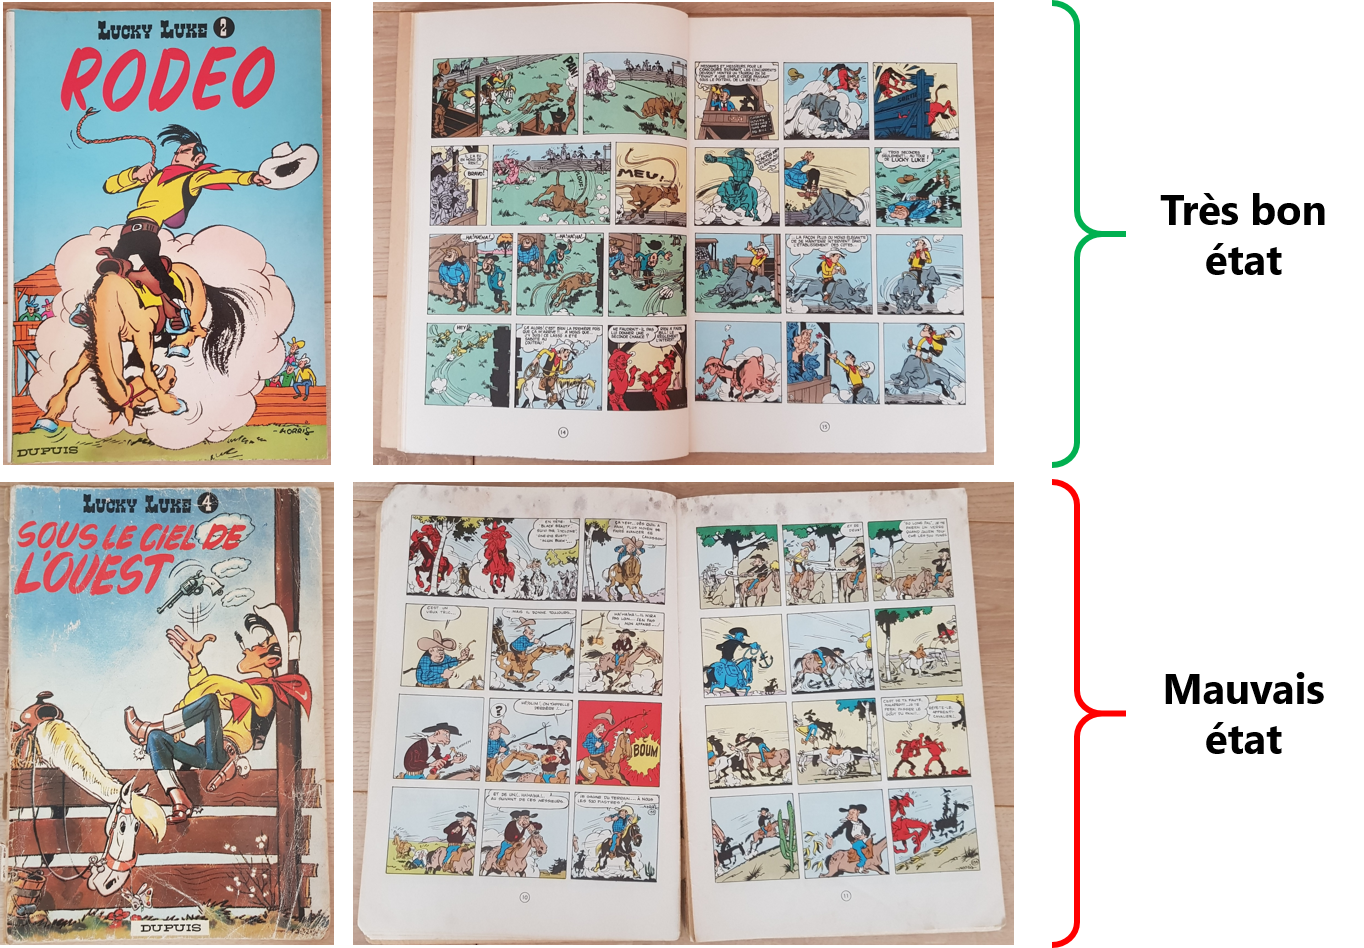
\includegraphics[width=0.80\textwidth]{figures/etatdelart-morris-1950-lucky-luke-2-1952-lucky-luke-4}
					\caption{
						Exemple d'annotation de l'état d'une \texttt{BD} (ici: \cite{morris-goscinny:1950:rodeo} et \cite{morris-goscinny:1952:sous-ciel-ouest}).
						La première est en très bon état (couverture comme neuve, tranches légèrement usées, pages intactes) tandis que la seconde est en mauvais état (couverture usée, dos abimée, traces sur les pages, ...).
					}
					\label{figure:2.1.2.B-PRESENTATION-ANNOTATION-EXEMPLES-CLASSIFICATION}
				\end{figure}
			\end{leftBarExamples}
			
			% Conclusion.
			Ainsi, si quelqu'un s'interroge sur l'état d'une bande dessinée en sa possession, ce modèle peut identifier l'état le plus probable d'après les exemples disponibles dans sa base d'apprentissage.
			
			% Autre cas d'usage similaire: Identifier la langue de la BD.
			\begin{leftBarInformation}
				De manière équivalente, il est possible de faire de la classification sur d'autres données, comme par exemple la classification de textes pour identifier la langue de l'ouvrage.
				Dans l'exemple ci-dessous, les catégories proposées sont "\texttt{Français}", "\texttt{Anglais}" et "\texttt{Allemand}", et la tâche d'annotation consiste ici à associer à chaque texte une catégorie de langue.
				\begin{center}
				\begin{tabular}{ c l }
					\textguillemets{\textit{
						Les cousins Dalton ont dévalisé la diligence.
					}} & $\implies$ \textcolor{colorSilverLakeBlue}{\texttt{Français}} \\
					\textguillemets{\textit{
						The Dalton cousins robbed the stagecoach.
					}} & $\implies$ \textcolor{colorDarkPastelGreen}{\texttt{Anglais}} \\
					\textguillemets{\textit{
						Die Dalton-Cousins haben die Postkutsche ausgeraubt.
					}} & $\implies$ \textcolor{colorDarkPastelRed}{\texttt{Allemand}}
				\end{tabular}
				\end{center}
			\end{leftBarInformation}
		
		
		%%% 2.1.2.C. Identification d'une bande dessinée à partir de sa couverture.
		\subsubsection{Identification d'une bande dessinée à partir de sa couverture.}
		\label{section:2.1.2.C-PRESENTATION-ANNOTATION-EXEMPLES-EXTRACTION}
			
			% Cas d'usage: identifier une bande dessinée
			Identifier une bande dessinée n'est pas toujours facile, et recopier l'ensemble des informations l'identifiant peut prendre du temps.
			Les libraires ou les collectionneurs désirant faire l'inventaire des ouvrages en leur possession peuvent ainsi y passer de nombreuses heures, avec le risque de faire des erreurs lors de l'inscription des bande dessinée dans leur registre.
			
			% Entrainer un modèle: extraction de caractères.
			Afin d'aider les collectionneurs, il est possible d'utiliser un modèle de \texttt{reconnaissance optique des caractères} (\texttt{OCR}) \footnote{
				Pour plus de détails sur l'\texttt{OCR}: voir la revue de \cite{berchmans-kumar:2014:optical-character-recognition} ou de \cite{awel-abidi:2019:review-optical-character}.
			} pour extraire automatiquement les informations importantes présentes sur les couvertures d'une \texttt{BD} à identifier.
			Pour entraîner un tel modèle, il est nécessaire d'avoir une base d'apprentissage contenant des exemples de pages de couverture avec la position et la valeur des informations pertinentes à extraire.
			La tâche d'annotation peut alors consister à renseigner pour chaque couverture de bande dessinée :
			\begin{itemize}
				\item la position des informations en l'encadrant sur l'image (avec un rectangle par exemple) ;
				\item la valeur écrite dans l'encadré sur l'image.
			\end{itemize}
			
			% Citation de l'exemple.
			Un exemple d'annotation de textes dans une image est disponible dans la \textsc{Figure~\ref{figure:2.1.2.C-PRESENTATION-ANNOTATION-EXEMPLES-EXTRACTION}}.
			%
			\begin{leftBarExamples}
				\begin{figure}[H]
					\centering
					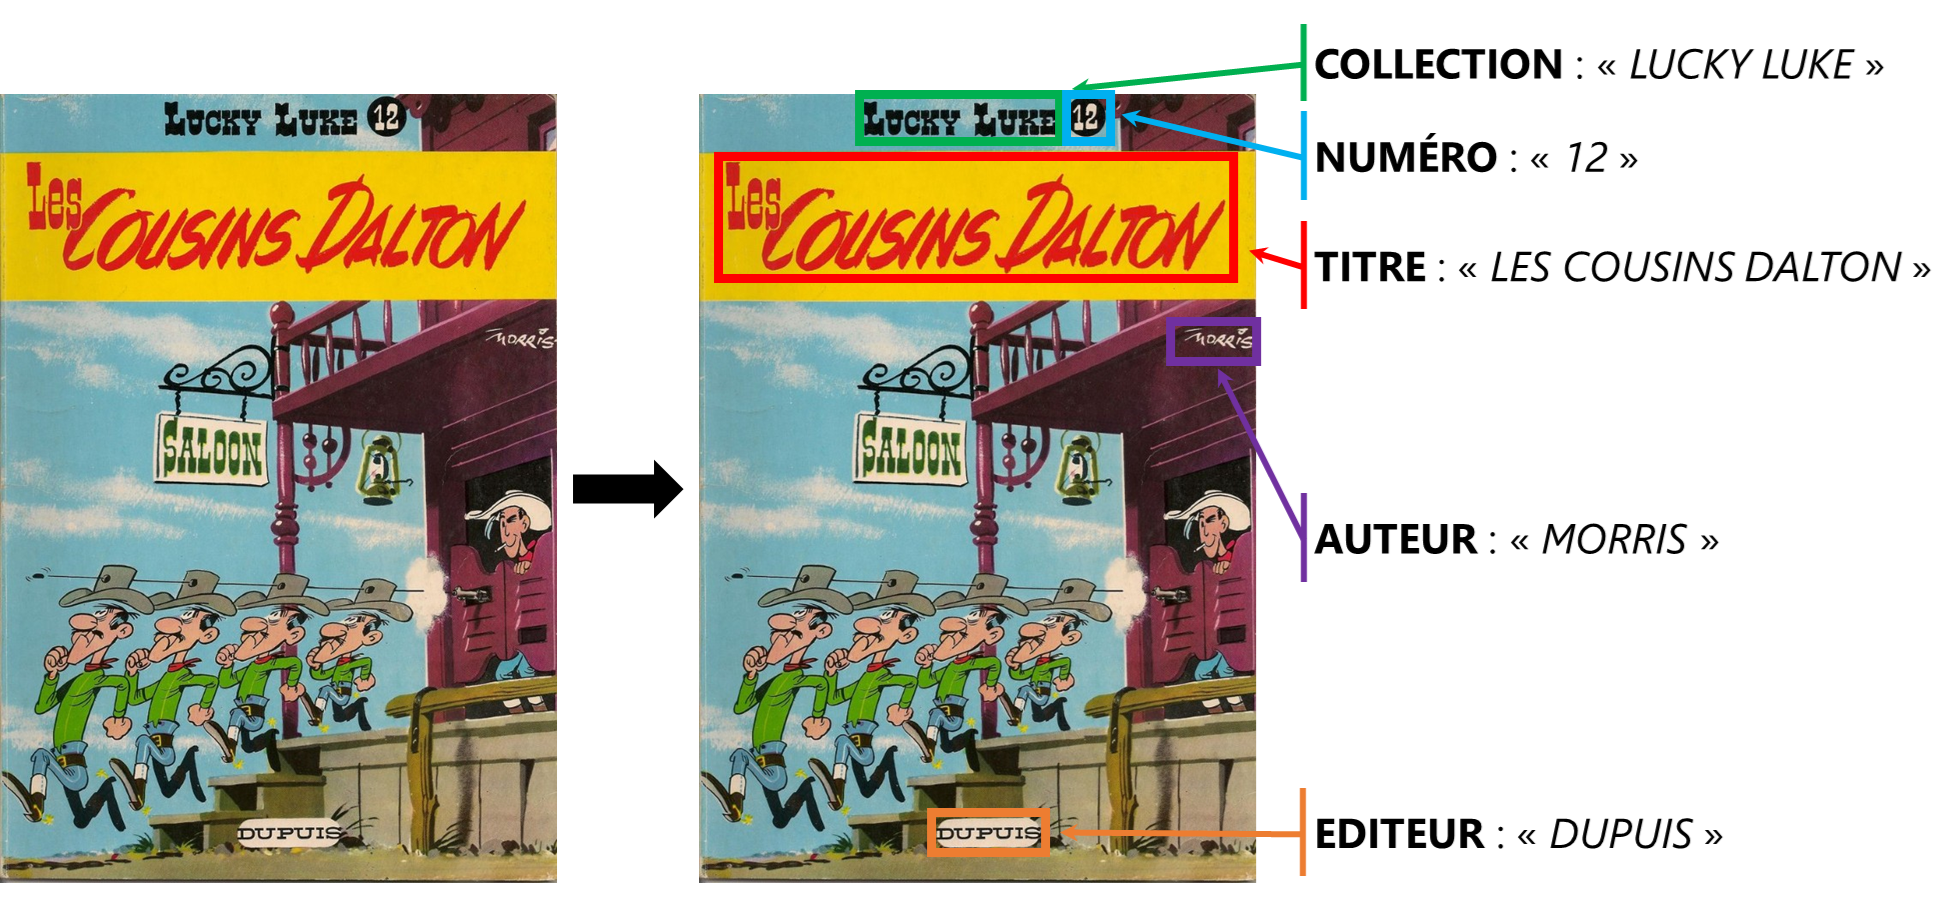
\includegraphics[width=0.80\textwidth]{figures/etatdelart-morris-1958-lucky-luke-12}
					\caption{
						Exemple d'annotation de textes présents sur la couverture d'une bande dessinée (ici: \cite{morris-goscinny:1958:cousins-dalton}).
						Les informations essentielles telles que la collection, le numéro, le titre, l'auteur et l'éditeur y sont présentes. 
					}
					\label{figure:2.1.2.C-PRESENTATION-ANNOTATION-EXEMPLES-EXTRACTION}
				\end{figure}
			\end{leftBarExamples}
			
			% Conclusion.
			Ainsi, si quelqu'un veut identifier une nouvelle bande dessinée, il peut interroger le modèle d'extraction de caractères pour récupérer les informations textuelles présentes dans la couverture, à l'image des exemples disponibles dans sa base d'apprentissage.
			
			% Autres cas d'usage: Extraire les information d'un texte.
			\setcounter{localCounterOfFootnoteValue}{\value{footnote}}
			\begin{leftBarInformation}
				De manière équivalente, il est possible de réaliser une \texttt{reconnaissance d'entités nommées (\texttt{NER})} \footnotemark pour extraire les informations citées dans un texte.
				Dans l'exemple ci-dessous, les types d'entités présentes sont "\texttt{personnage}", "\texttt{métier}", "\texttt{argent}", "\texttt{lieu}" et "\texttt{date}".
				La tâche d'annotation consiste ici à identifier la position et le type de chaque entité présente.
				
				\begin{quote}
					\textguillemets{\textit{
						$\textbf{\text{Lucky Luke}}_{\textcolor{colorDarkPastelRed}{\texttt{(personnage)}}}$, le $\textbf{\text{cow-boy}}_{\textcolor{colorDarkPastelPurple}{\texttt{(métier)}}}$ solitaire, a attrapé les $\textbf{\text{Dalton}}_{\textcolor{colorDarkPastelRed}{\texttt{(personnage)}}}$ à $\textbf{\text{Coyote Gulch}}_{\textcolor{colorCarrotOrange}{\texttt{(lieu)}}}$ et a touché $\textbf{\text{50.000\$}}_{\textcolor{colorSilverLakeBlue}{\texttt{(argent)}}}$ en les livrant au $\textbf{\text{pénitencier}}_{\textcolor{colorCarrotOrange}{\texttt{(lieu)}}}$. Ils se sont évadés le $\textbf{\text{jeudi suivant}}_{\textcolor{colorDarkPastelGreen}{\texttt{(date)}}}$.
					}}
				\end{quote}
			\end{leftBarInformation}
			% Rattraper les footnote.
				\stepcounter{localCounterOfFootnoteValue}
				\footnotetext[\value{localCounterOfFootnoteValue}]{
					Pour plus de détails sur la reconnaissance d'entités nommées (\texttt{NER}): voir les revues de \cite{goyal-etal:2018:recent-named-entity} ou de \cite{li-etal:2022:survey-deep-learning}.
				}
		
		
		%%% 2.1.2.D. Interprétation audio d'une bande dessinée.
		\subsubsection{Interprétation audio d'une bande dessinée.}
		\label{section:2.1.2.D-PRESENTATION-ANNOTATION-EXEMPLES-TRANSCRIPTION}
		
			% Cas d'usage: générer une lecture audio.
			Il est de plus en plus commun de trouver des livres disponibles avec une lecture audio.
			Ces audio-livres, réalisés par une personne ou synthétisés par l'ordinateur, peuvent être à visée éducative ou simplement disponibles pour le loisir.
			Dans le cadre de notre exemple sur le thème des bandes dessinées, peu d'entre elles disposent d'une lecture audio.
			Une idée serait donc d'interpréter une lecture audio de ces bandes dessinées en synthétisant la voix des doubleurs de leurs adaptations télévisées (ou simplement d'un narrateur si l'oeuvre n'a pas été portée à l'écran).
			
			% Entrainer un modèle: synthétiseur vocal.
			Dans le but de créer ces audio-\texttt{BD}, nous pourrions envisager d'utiliser des modèles de \texttt{synthèse vocale} (\texttt{TTS}) \footnote{
				Pour plus de détails sur la synthèse vocale: voir la revue de \cite{kothadiya-etal:2020:different-methods-review} ; voir un exemple d'architecture neuronale \texttt{end-to-end} dans \cite{mu-etal:2021:review-endtoend-speech}.
			} pour générer automatiquement la lecture des bulles d'une bande dessinée.
			Pour entraîner de tels modèles, il est nécessaire d'avoir une base d'apprentissage contenant des exemples d'audios prononcés par chacun des personnages (ici: les doubleurs de l'adaptation télévisée) avec la transcription de leur paroles pour chaque audio.
			La tâche d'annotation peut alors consister à renseigner le personnage et les paroles qu'il a prononcées.
			
			% Citation de l'exemple.
			Un exemple d'annotation phonétique est illustré dans la \textsc{Figure~\ref{figure:2.1.2.D-PRESENTATION-ANNOTATION-EXEMPLES-TRANSCRIPTION}}.
			%
			\begin{leftBarExamples}
				\begin{figure}[H]
					\centering
					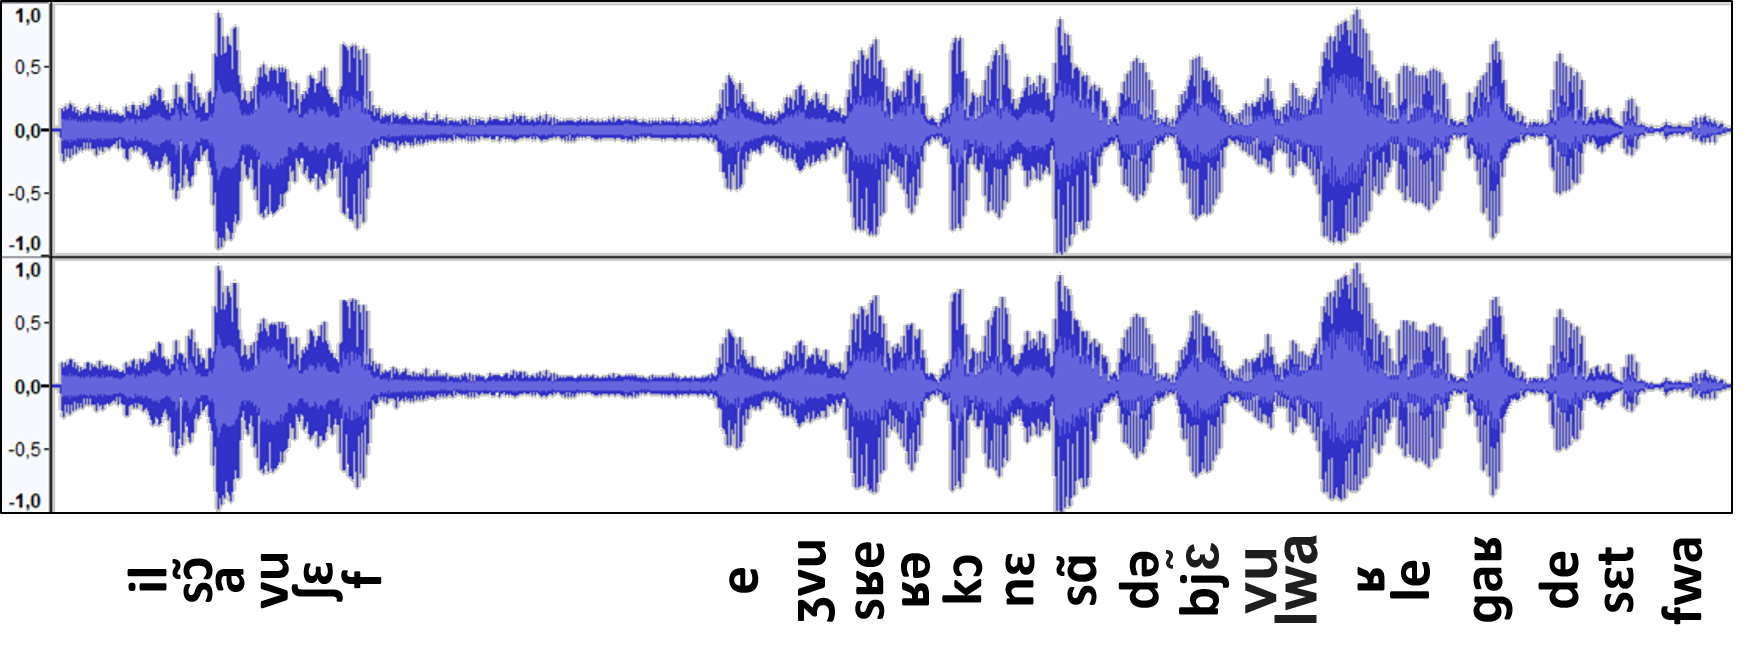
\includegraphics[width=0.95\textwidth]{figures/etatdelart-thebault-transcription}
					\caption{
						Exemple de paroles prononcées dans un audio.
						Ici, la voix de \textit{Lucky Luke} est interprétée par Jacques THEBAULT.
						Le texte annoté, c'est-à-dire celui prononcé dans l'audio, est  \textguillemets{\texttt{Ils sont à vous chef, et j'vous s'rai reconnaissant de bien les garder cette fois.}}.
						Les phonèmes en alphabet phonétique international associés à chaque séquence de l'audio sont disponibles si besoin.
						%[il sɔ̃ a vu ʃɛf, e ʒvu sʁe ʁə.kɔ.nɛ.sɑ̃ də bjɛ̃ vu.lwaʁ le ɡaʁ.de sɛt fwa].
					}
					\label{figure:2.1.2.D-PRESENTATION-ANNOTATION-EXEMPLES-TRANSCRIPTION}
				\end{figure}
			\end{leftBarExamples}
			
			% Conclusion.
			Ainsi, nous pourrions consulter le modèle de synthèse vocale d'un personnage (ici: celui de \texttt{Lucky Luke}) avec un nouveau texte à prononcer pour en obtenir une lecture audio dont la voix se rapproche des enregistrements de la base d'apprentissage (ici: celle de Jacques THEBAULT).
			
			% Autres cas d'usage: comuler OCR + Classification + TTS
			\begin{leftBarInformation}
				Nous pourrions compléter le cas d'usage
				(1) en extrayant automatiquement le texte d'une planche de \texttt{BD} par \texttt{OCR},
				(2) en détectant automatiquement le personnage prononçant la bulle de \texttt{BD} par classification,
				puis (3) en générant du texte à prononcer par le personnage par synthèse vocale.
				Bien entendu, la conception et l'enchaînement de ces différents modèles sont plutôt complexes, et chaque tâche de \textit{Machine Learning} demande ses propres données annotées pour construire une base d'apprentissage.
			\end{leftBarInformation}
			
			
		%%% Exemple: Annotation génération musicale
		% Generation de musique: \cite{hernandez-olivan-beltran:2023:music-composition-deep}
		%\begin{leftBarExamples}
		%	Annotation des paroles d'une chanson (\cite{woods:1971:poor-lonesome-cowboy}). \\
		%
		%	\begin{guitar}
		%		\textbf{Im A Poor Lonesome Cowboy}
		%		\textit{
		%			~~~~from \texttt{Lucky Luke - Daisy Town OST} ($1971$)
		%			~~~~composed by \texttt{Claude Bolling}
		%			~~~~performed by \texttt{Pat Woods}
		%		}
		%		\texttt{Intro}
		%		\textit{
		%			[D]Lonesome [D7]cowboy, [G]Lonesome [G7]cowboy, [D]You're a [Bm]long [Bm7]long [E]way from [A]home.
		%			[D]Lonesome cowboy, [G]Lonesome cowboy, [D]You've a [Bm]long [Bm7]long [E]way [A7]to [D]roam.
		%		}
		%		\texttt{Couplet}
		%		\textit{
		%			I'm a [D]poor lonesome cowboy, I'm a long long way from home,
		%			And this poor lonesome [F\#m]cowboy, Has got a [Em]long long way [A]to roam.
		%			Over [D]mountains and over [D7]prairies, From [G]dawn 'til day is [Em]done,
		%			My [Bm]horse and me keep [F\#]ridin', [G]into the [A]settin' [D]sun.
		%		}
		%		{ \center \textbf{...} }
		%	\end{guitar}
		%\end{leftBarExamples}
		
		
		%%% Exemple: Annotation étiquette gramaticale
		%\begin{leftBarExamples}
		%	Annotation des étiquettes grammaticales dans un texte.
		%	\begin{quote}
		%		\textguillemets{\textit{
		%			$\text{Les}_{\textcolor{colorDarkPastelPurple}{\texttt{(DET)}}}$
		%			$\text{dangereux}_{\textcolor{colorMinionYellow}{\texttt{(ADJ)}}}$
		%			$\text{Dalton}_{\textcolor{colorDarkPastelRed}{\texttt{(PROPN)}}}$
		%			$\text{se}_{\textcolor{colorCarrotOrange}{\texttt{(PRON)}}}$
		%			$\text{sont}_{\textcolor{colorDarkPastelGreen}{\texttt{(AUX)}}}$
		%			$\text{encore}_{\textcolor{colorSilverLakeBlue}{\texttt{(ADV)}}}$
		%			$\text{évadés}_{\textcolor{colorDarkPastelGreen}{\texttt{(VERB)}}}$
		%			$\text{de}_{\textcolor{colorDimGray}{\texttt{(ADP)}}}$
		%			$\text{prison}_{\textcolor{colorDarkPastelRed}{\texttt{(NOUN)}}}$
		%			$\text{et}_{\textcolor{colorBlack}{\texttt{(CCONJ)}}}$
		%			$\text{ils}_{\textcolor{colorCarrotOrange}{\texttt{(PRON)}}}$
		%			$\text{ont}_{\textcolor{colorDarkPastelGreen}{\texttt{(AUX)}}}$
		%			$\text{déjà}_{\textcolor{colorSilverLakeBlue}{\texttt{(ADV)}}}$
		%			$\text{dévalisé}_{\textcolor{colorDarkPastelGreen}{\texttt{(VERB)}}}$
		%			$\text{une}_{\textcolor{colorDarkPastelPurple}{\texttt{(DET)}}}$
		%			$\text{banque}_{\textcolor{colorDarkPastelRed}{\texttt{(NOUN)}}}$
		%			$\text{à}_{\textcolor{colorDimGray}{\texttt{(ADP)}}}$
		%			$\text{Daisy Town}_{\textcolor{colorDarkPastelRed}{\texttt{(PROPN)}}}$.
		%		}}\\
		%		%{ \center \scriptsize (
		%		%	Adjectif: {\textcolor{colorMinionYellow}{\texttt{(ADJ)}}} ;
		%		%	Adverbe: {\textcolor{colorSilverLakeBlue}{\texttt{(ADV)}}} ;
		%		%	Conjonction: {\textcolor{colorBlack}{\texttt{(CCONJ)}}} ;
		%		%	Déterminant: {\textcolor{colorDarkPastelPurple}{\texttt{(DET)}}} ;
		%		%	Nom: {\textcolor{colorDarkPastelRed}{\texttt{(NOUN)}}}, {\textcolor{colorDarkPastelRed}{\texttt{(PROPN)}}} ;
		%		%	Préposition: {\textcolor{colorDimGray}{\texttt{(ADP)}}} ;
		%		%	Pronom: {\textcolor{colorCarrotOrange}{\texttt{(PRON)}}}, ;
		%		%	Verbe: {\textcolor{colorDarkPastelGreen}{\texttt{(AUX)}}}, {\textcolor{colorDarkPastelGreen}{\texttt{(VERB)}}}.
		%		%)}
		%	\end{quote}
		%\end{leftBarExamples}
	
	
	%%%
	%%% Subsection 2.1.3: Bilan concernant la présentation de l'annotation.
	%%%
	\subsection{Bilan concernant la présentation de l'annotation}
	\label{section:2.1.3-PRESENTATION-ANNOTATION-BILAN}
	
	%%%
	%%% Conclusion.
	%%%
	\begin{leftBarSummary}
		\begin{todolist}
			% Définition de l'annotation.
			\item[\itemok] \textguillemets{\texttt{Annoter}} une donnée consiste à \textbf{ajouter un complément d'information} pour pouvoir mieux interpréter puis reproduire un phénomène.
			% Type d'annotation.
			\item[\itemok] Le type d'annotation à réaliser \textbf{dépend du problème à traiter} : régression, classification, extraction d'information, génération ou synthèse de données, ...
			% Corpus d'entraînement.
			\item[\itemok] L'ensemble des données annotées peut être utilisé pour concevoir un modèle d'\textguillemets{\texttt{apprentissage automatique}}: il est alors appelé \textguillemets{\texttt{corpus d'entraînement}}.
		\end{todolist}
	\end{leftBarSummary}